%!TEX root = ./template-skripsi.tex
%-------------------------------------------------------------------------------
%                            	BAB IV
%               		KESIMPULAN DAN SARAN
%-------------------------------------------------------------------------------

\chapter{HASIL DAN PEMBAHASAN}

Pada bab ini akan dibagi ke dalam dua bagian yaitu pengkodean dan hasil. Pada bagian pengkodean akan dibahas implementasi algoritma ke dalam kode pemrograman. Selanjutnya pada bagian hasil akan dijelaskan hasil pengujian program terhadap data yang dipakai sehingga dapat dibuat sebuah kesimpulan pada bab selanjutnya.

\section{Pengkodean}

Akan dibahas implementasi algoritma ke dalam kode pemrograman Python. Program dapat dipisah menjadi empat bagian, yaitu tiga bagian berbeda berdasarkan algoritma yang dipakai dan bagian kode program yang dipakai bersama (\textit{shared code}). Pada bagian kode program bersama, terdapat \textit{Helper Class} yang bertugas untuk \textit{caching} dan mengakses basis data atau \textit{Helper Function} yang melakukan tugas umum seperti perhitungan matematika, mengambil alamat \textit{domain} dari \textit{string url}.

\subsection{\textit{Shared Code}}

Untuk melakukan \textit{caching}, \textit{library} Pickle dipakai. Pickle mengubah objek pada program menjadi \textit{byte stream} yang disimpan ke dalam \textit{file} berformat ".pkl". Tujuan dilakukan \textit{caching} ini untuk meringankan penggunaan memori utama dengan menyimpan objek ke \textit{disk}, dan hanya dimuat ke memori utama ketika hanya akan digunakan. Objek-objek yang disimpan ke dalam \textit{cache} adalah matriks $P$ yang dipecah berdasarkan kolomnya, matriks $Q$, matriks $P_{ii}$, matriks $P_{i*}$, matriks $P_{*i}$, dan matriks $RP$. 

Potongan kode \ref{listing:caching_class} berisi \textit{class} untuk \textit{caching} \textit{Class} Cache merupakan \textit{Parent Class} dari PCache, yang sesuai namanya, bertugas melakukan \textit{Caching} untuk matriks $P$. Selain PCache juga ada \textit{Cache Class} lain seperti, QListCache untuk matriks $Q$, PiiListCache untuk matriks $P_{ii}$, PiastListCache untuk matriks $P_{i*}$, PastiListCache untuk matriks $P_{*i}$, dan RPCache untuk matriks $RP$. Secara garis besar \textit{class} tersebut memiliki \textit{method} dan \textit{property} yang mirip, seperti nama \textit{file}, dan \textit{method} untuk menyimpan dan memuat \textit{cache}.

\begin{figure}[H]
  \centering
  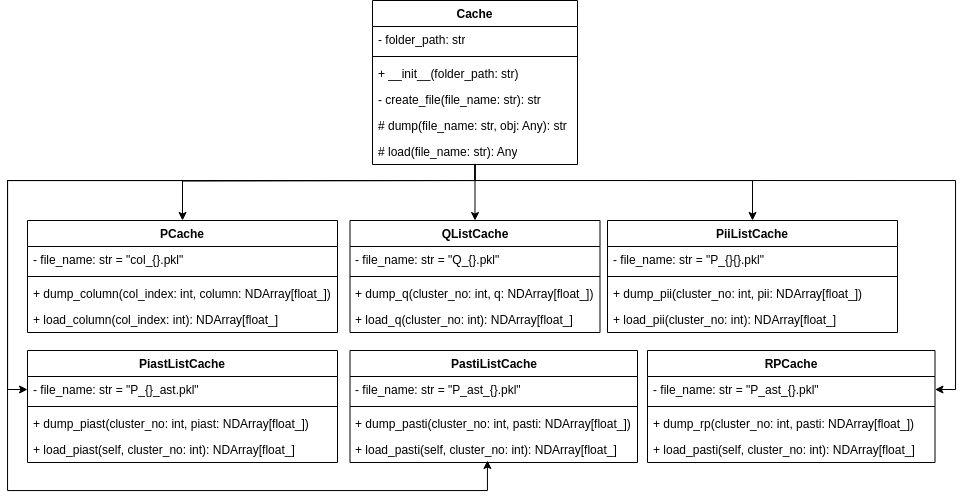
\includegraphics[keepaspectratio, width={\textwidth}]{gambar/cache_class_diagram}
  \caption{\textit{Class Diagram} dari \textit{class} Cache dan turunannya}
	\label{gambar:cache_class_diagram}
\end{figure}

Selanjutnya terdapat \textit{Class} yang bertugas menghubungkan basis data ke program. \textit{Class} DB merupakan \textit{Class} dasar untuk mengurus koneksi basis data ke program. \textit{Class} DB dibungkus ke dalam \textit{Repository Class} yang dibatasi oleh tabel tertentu dengan maksud agar tidak ada \textit{Class} yang terlalu besar karena bertanggung jawab pada banyak tugas. Sebagai contoh pada \textit{Class} PageInformationRepository bertugas mengurus tabel \textit{page\_information}. PageInformationRepository memiliki \textit{method} \textit{get\_all\_page\_informations}, sesuai namanya, mengambil semua baris dari tabel \textit{page\_information} dan dikembalikan dalam bentuk List yang berisi \textit{Class} PageInformation (lihat kode \ref{listing:db.py} dan kode \ref{listing:page_information_repository.py}). Selain PageInformationRepository, juga ada \textit{Repository Class} lain seperti PageLinkingRepository yang tugas utamanya mengambil data tabel \textit{page\_linking}, dan PagerankRepository yang tugas utamanya memasukan data hasil \textit{ranking} halaman ke tabel \textit{page\_rank\_original\_pagerank\_dpc\_paper\_version}, \textit{page\_rank\_dpc}, dan \textit{page\_rank\_modified\_dpc\_v2}.

\begin{figure}[H]
  \centering
  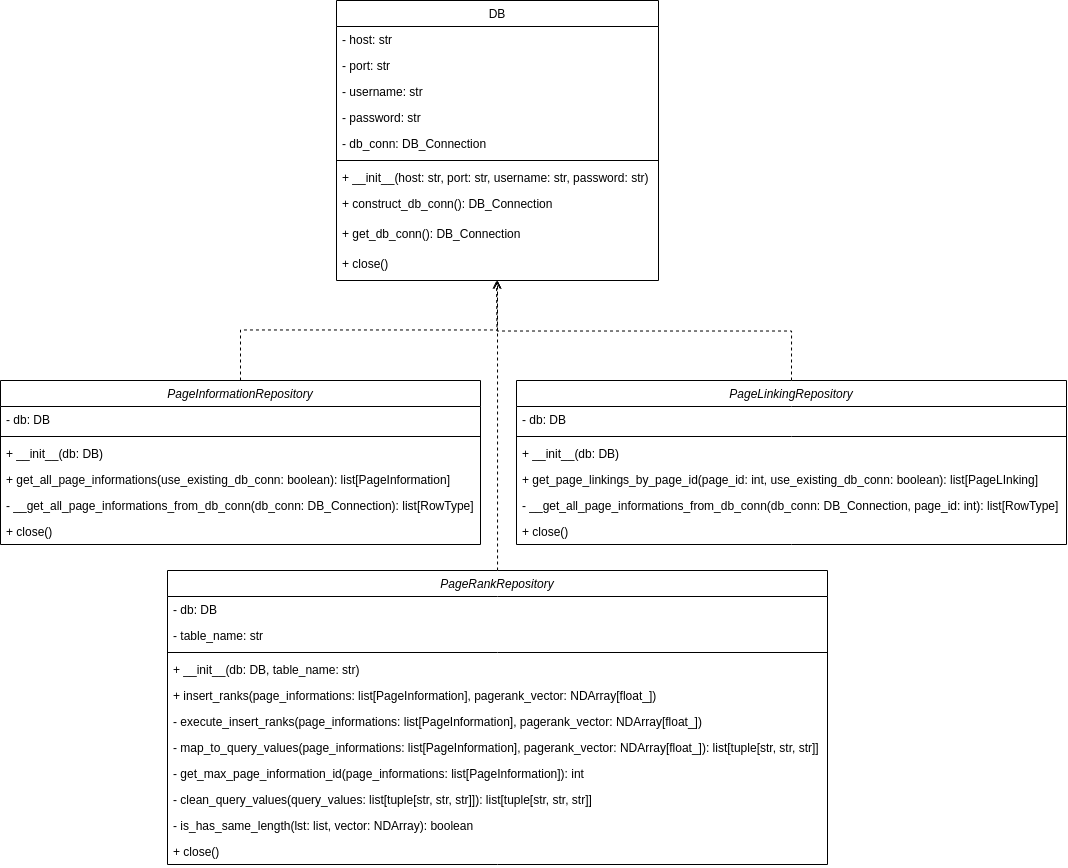
\includegraphics[keepaspectratio, width={\textwidth}]{gambar/db_class_diagram}
  \caption{\textit{Class Diagram} dari \textit{class} DB dan \textit{class} lain yang memiliki dependensi terhadapnya}
	\label{gambar:db_class_diagram}
\end{figure}

Sebelumnya sempat disinggung \textit{Class} PageInformation tanpa penjelasan lebih lanjut. \textit{Class} PageInformation merupakan salah satu dari dua \textit{Model Class} yang ada di program penelitian ini. \textit{Model Class} merupakan \textit{Class} sederhana yang memodelkan data pada program. Pada kode \ref{listing:model.py} terdapat PageInformation dan PageLinking. PageInformation menampung data baris pada tabel \textit{page\_information}. PageInformation memiliki tiga atribut yaitu \textit{index} urutan PageInformation dalam matriks, \textit{id\_page} yang diambil dari basis data, dan url yang juga diambil dari basis data. Yang kedua ada PageLinking menampung data baris pada tabel \textit{page\_linking} yang memiliki atribut \textit{outgoing\_link} yang diambil dari basis data.

Pada kode \ref{listing:helper_functions.py} terlihat \textit{helper functions} yang memiliki kegunaan tertentu yang bersifat umum. Sebagai contoh fungsi \textit{l1\_norm} mengembalikan nilai \textit{l1 norm} dari suatu List. Selanjutnya ada \textit{create\_url\_to\_page\_information\_dict} yang mengubah List yang berisi PageInformation menjadi sebuah \textit{dictionary} dengan \textit{url} sebagai kunci, dan PageInformation merupakan isinya. Fungsi \textit{sort\_page\_information\_by\_domain} mengurutkan List PageInformation berdasarkan domain-nya. Selain \textit{helper functions}, di \textit{file} yang sama, juga ada \textit{class} PageInformationClusterizer yang tugasnya adalah mengelompokan List yang berisi PageInformation berdasarkan domain-nya, hasil akhirnya adalah sebuah \textit{dictionary} yang \textit{key}-nya merupakan domain, dan \textit{value}-nya merupakan List PageInformation yang sudah dikelompokan sebelumnya.

\begin{figure}[H]
  \centering
  
\includegraphics[keepaspectratio, width={\textwidth}]{gambar/page_information_clusterizer_class_diagram}
  \caption{\textit{Class Diagram} dari \textit{class} PageInformationClusterizer}
	\label{gambar:page_information_clusterizer_class_diagram}
\end{figure}

\textit{Class} PHelper adalah sebuah \textit{class} yang bertugas untuk membuat matriks transisi $P$. \textit{Class} PHelper memiliki dependensi terhadap \textit{class} PageLinkingRepository karena untuk menentukan nilai elemennya didasari pada \textit{link} pada halaman web. Kode dan \textit{Class Diagram} PHelper secara berurutan dapat dilihat pada kode \ref{listing:PHelper.py} dan gambar \ref{gambar:p_helper_class_diagram_2}.

\begin{figure}[H]
\centering
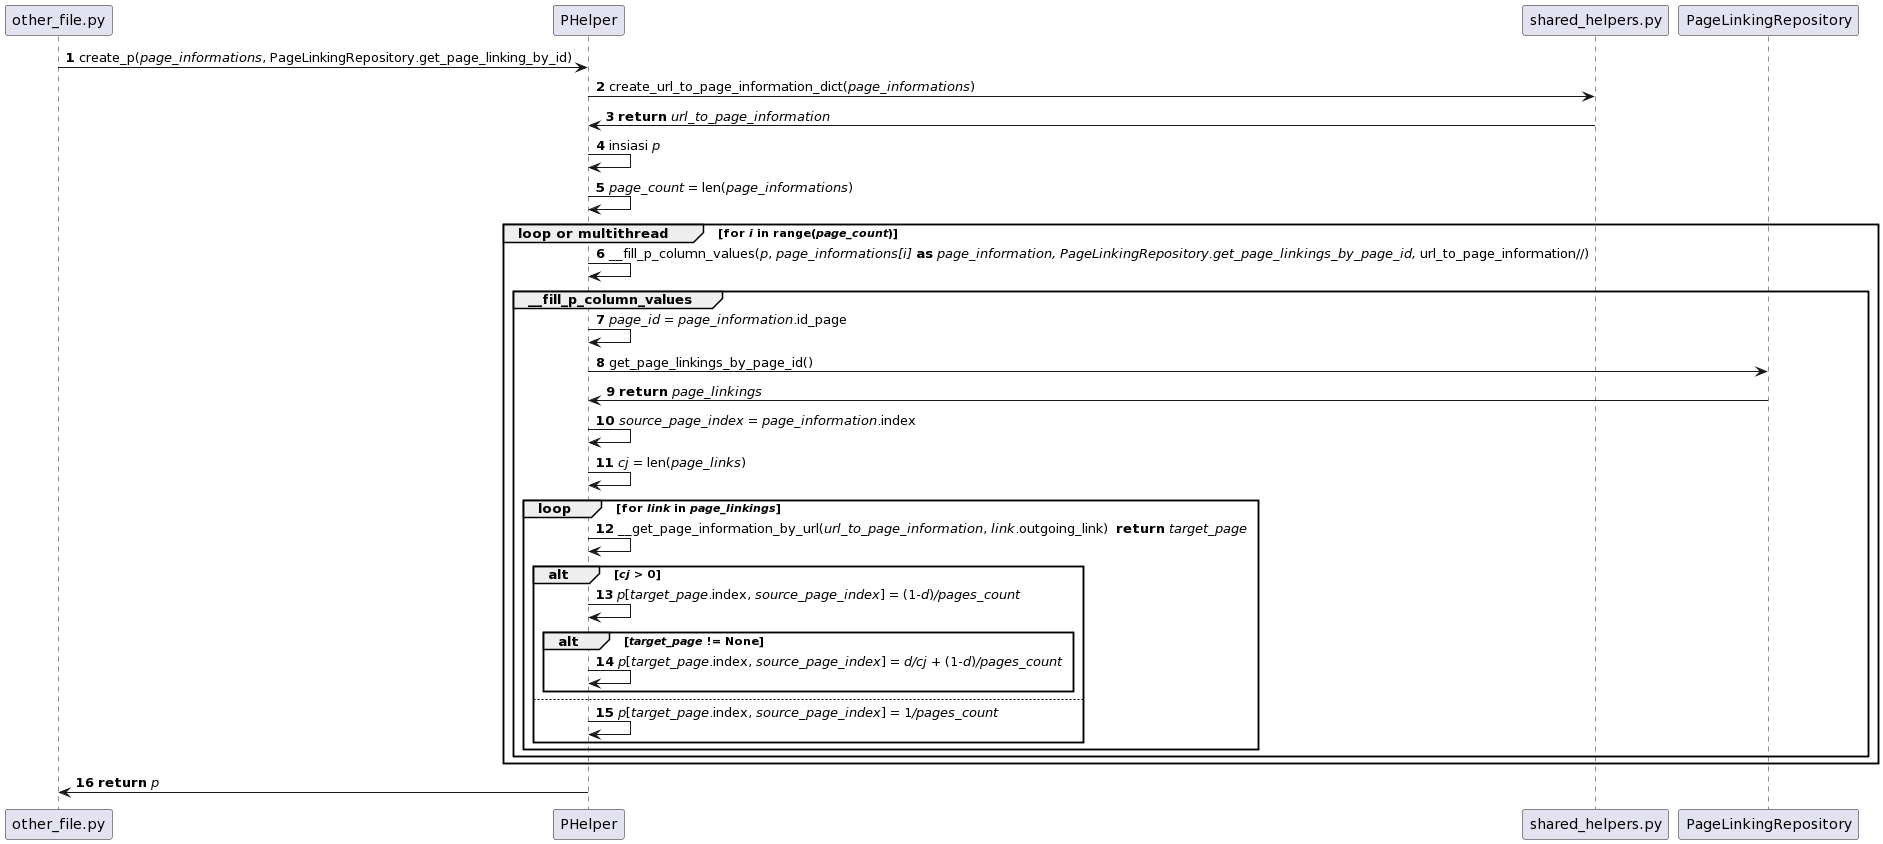
\includegraphics[width={\textheight}, height={\textwidth}, angle=270]{gambar/p_helper_sequence_diagram_2}
\caption{Diagram alir ketika membentuk matriks transisi $P$ di \textit{class} PHelper}
\label{gambar:p_helper_sequence_diagram_2}
\end{figure}

\begin{figure}[H]
\centering
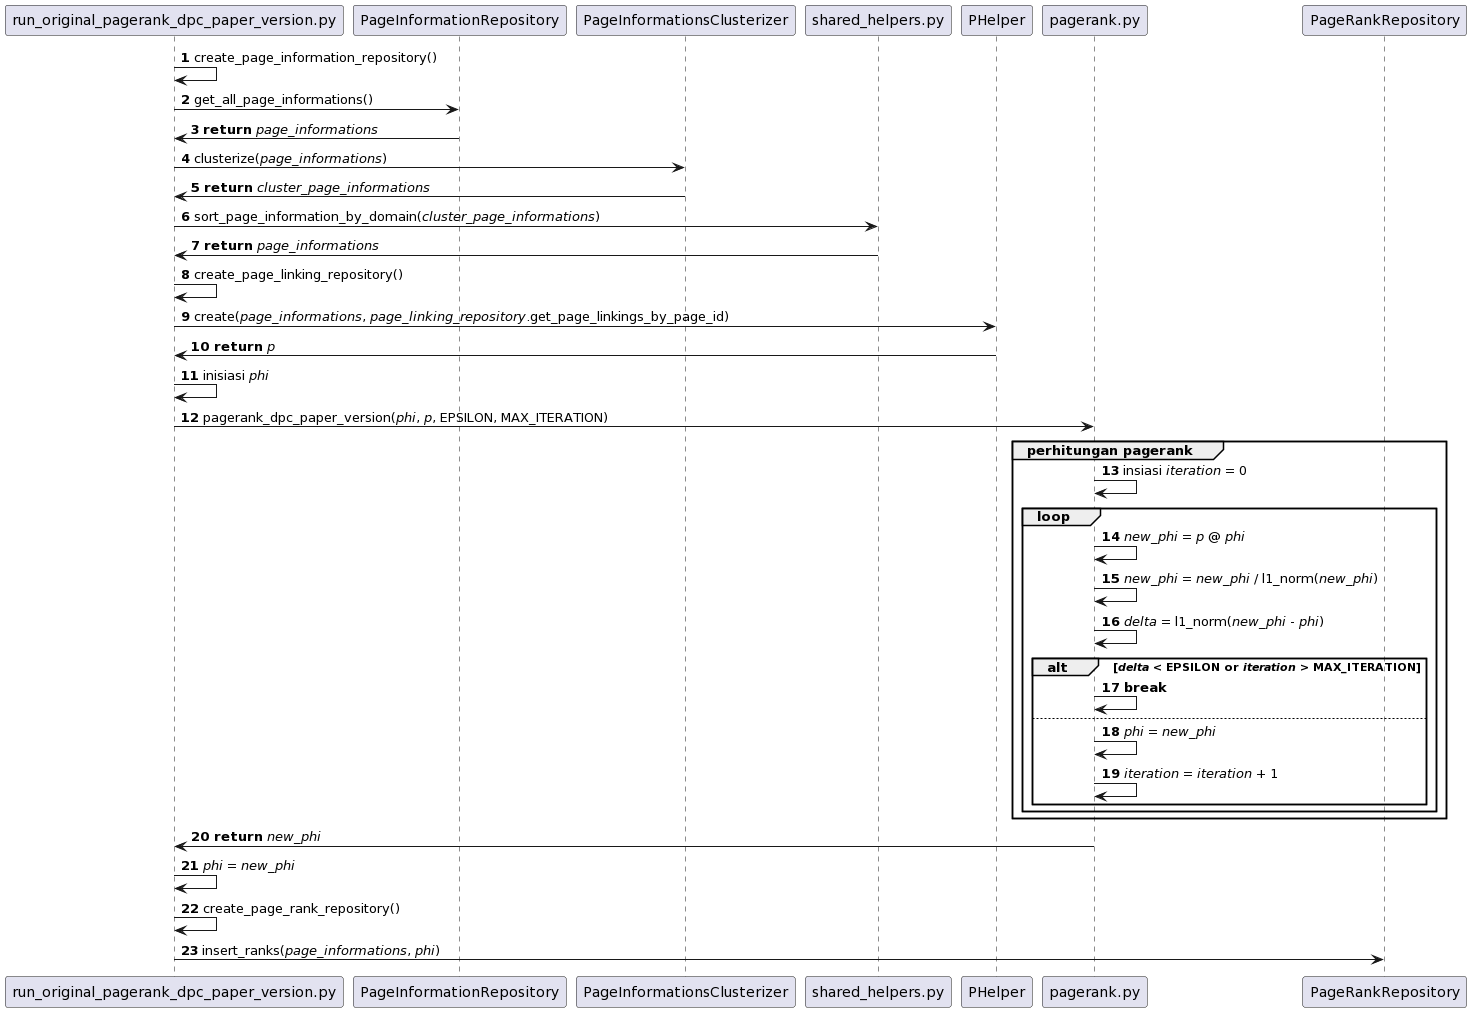
\includegraphics[width={\textheight}, height={\textwidth}, angle=270]{gambar/run_original_pagerank_dpc_paper_version_sequence_diagram}
\caption{Diagram alir dari program Pagerank}
\label{gambar:run_original_pagerank_dpc_paper_version_sequence_diagram}
\end{figure}

\begin{figure}[H]
\centering
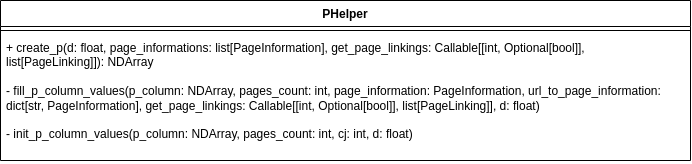
\includegraphics[keepaspectratio, width={\textwidth}]{gambar/p_helper_class_diagram(2)}
\caption{\textit{Class Diagram} PHelper}
\label{gambar:p_helper_class_diagram_2}
\end{figure}

Alur kerja dari PHelper dapat dilihat pada diagram alir \ref{gambar:p_helper_sequence_diagram_2}. Kotak abu-abu pada kiri dan kanan diagram menunjukan nama \textit{file} atau \textit{class} terjadinya proses, tanda panah menunjukan perpindahan alur eksekusi dari \textit{file}/\textit{class} yang satu ke yang lainnya, nama di atas panah merupakan nama \textit{method} atau \textit{function} yang dipanggil, kata "\textit{return}" berarti hasil keluaran dari \textit{method}/\textit{function}, kata "\textit{loop}" berarti pengulangan, kata "\textit{alt}" berarti percabangan alur program. Pada langkah satu \textit{method} \textit{create\_p} dipanggil dengan argumen \textit{page\_informations} dan sebuah \textit{method} \textit{PageLinkingRepository.get\_page\_linking\_by\_id}. Pada langkah dua dibuat sebuah \textit{dictionary} yang berisi PageInformation dan \textit{url}-nya sebagai kunci. Selanjutnya pada langkah enam, dilakukan \textit{looping} berdasarkan jumlah banyaknya halaman web yang ada pada \textit{dataset}, proses ini juga dapat dilakukan secara pararel dengan \textit{multi threading}. Pada langkah enam dilakukan pengisian matriks $P$ pada setiap kolomnya. Alasan dilakukan pada tiap kolom karena terdapat nilai yang dipakai secara bersama yaitu banyaknya jumlah \textit{PageLinking} suatu halaman web. Langkah 12 merupakan langkah penting, yaitu perhitungan nilai elemen matriks $P$. Dasar dari perhitungan dari persamaan \ref{eq:5-1}.

\subsection{Program Pagerank}

Alur algoritma Pagerank dalam program dapat dilihat pada gambar \ref{gambar:run_original_pagerank_dpc_paper_version_sequence_diagram}. Langkah satu dilakukan instansiasi PageInformationRepository untuk mengambil semua data dari tabel \textit{page\_information} dari basis data. Selanjutnya pada langkah empat dilakukan klasterisasi dari data \textit{page\_information} untuk dilakukan pengurutan berdasarkan \textit{cluster}-nya. Hal ini dilakukan untuk mempermudah proses pemetaan antara vektor \textit{ranking} halaman web $\pi$ dengan \textit{list} \textit{page\_information}. Pada langkah delapan dilakukan instansiasi PageLinkingRepository untuk membuat matriks transisi $P$ yang memerlukan koneksi basis data untuk memperoleh data dari tabel \textit{page\_linking}. Setelah membuat matriks $P$, pada langkah sepuluh dilakukan inisiasi nilai $\pi$ dan $e$, dan selanjutnya dilakukan perhitungan \textit{pagerank}. Setelah melakukan perhitungan \textit{pagerank}, pada langkah 22 dilakukan instansiasi PagerankRepository, untuk menyimpam hasil perhitungan \textit{pagerank} ke basis data.

\subsection{Program DPC}

\quad Selanjutnya akan dibahas kode program DPC. Berbeda dengan program Pagerank yang cenderung lebih sederhana, perhitungan pada program DPC lebih kompleks. Akibatnya dibutuhkan \textit{class} pendukung yang lebih banyak. Terdapat delapan \textit{class} pendukung yang dipakai oleh program DPC, yaitu ClusterSeparatedPhiHelper, ExtendedLocalTransitionMatrixHelper, PWithCacheHelper, PartitionedPHelper, PastiHelper, PiastHelper, RPHelper, dan DPCExecutor.

ClusterSeparatedPhiHelper merupakan salah satu \textit{helper class} yang berisi \textit{method}-\textit{method} yang berkaitan dengan vektor $\pi$ yang dipecah sesuai dengan \textit{cluster}-nya masing-masing. \textit{Method} \textit{construct\_cluster\_separated\_phi} melakukan perhitungan pada langkah \ref{alg:3.step:trivial:2} pada algoritma DPC, menghitung nilai $\pi$ pada tiap \textit{cluster}. Selanjutnya \textit{method} \textit{flatten\_cluster\_separated\_phi} menyatukan vektor-vektor $\pi$ yang terpisah menjadi ke dalam satu vektor. \textit{Method} \textit{update\_cluster\_separated\_phi} melakukan perhitungan untuk memperbaharui nilai vektor $\pi$ sesuai dengan langkah \ref{alg:3.step:3:3} pada algoritma DPC. Yang terakhir ada \textit{method} \textit{construct\_s} yang membuat sebuah matriks $S$ berdasarkan vektor-vektor $\pi$ yang terpisah berdasarkan \textit{cluster}-nya.

\begin{figure}[H]
  \centering
  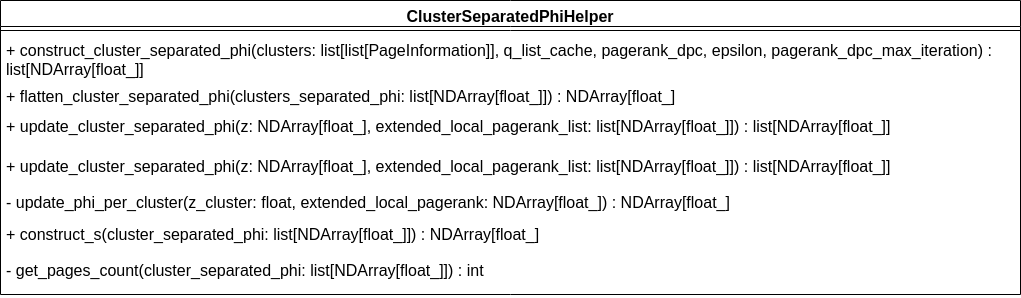
\includegraphics[keepaspectratio, width={\textwidth}]{gambar/cluster_separated_phi_helper_class_diagram}
  \caption{\textit{Class Diagram} ClusterSeparatedPhiHelper}
	\label{gambar:cluster_separated_phi_helper_class_diagram}
\end{figure}

\begin{figure}[H]
  \centering
  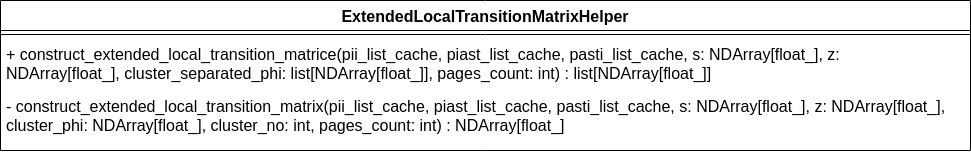
\includegraphics[keepaspectratio, width={\textwidth}]{gambar/extended_local_transition_matrix_helper_class_diagram}
  \caption{\textit{Class Diagram} ExtendedLocalTransitionMatrixHelper}
	\label{gambar:extended_local_transition_matrix_helper_class_diagram}
\end{figure}

ExtendedLocalTransitionMatrixHelper, sesuai namanya, merupakan \textit{helper class} yang berkaitan dengan matriks \textit{extended local transition matrix} yang dalam algoritma DPC berada pada langkah \ref{eq:9}. Pada \textit{method} \textit{construct\_extended\_local\_transition\_matrice} membentuk himpunan matriks $B$ pada setiap \textit{cluster}. Sesuai dengan langkah \ref{eq:9} pada algoritma DPC, \textit{method} ini memuat matriks $P_{ii}$ yang sudah di-\textit{caching} untuk dimasukkan ke beberapa kolom dan baris pertama matriks $B$. Selanjutnya, pada baris paling bawah diisi hasil perkalian vektor $e$ dan matriks $P_{*i}$ yang dimuat dari \textit{class} PastiListCache. Selanjutnya pada kolom paling kanan dilakukan perhitungan yang cukup panjang sesuai pada langkah \ref{eq:9} algoritma DPC. Sel kanan bawah matriks $B$ dapat bernilai apa saja, selama nilai total dari kolom paling kanan matriks $B$ bernilai satu.

Selanjutnya, PWithCacheHelper, sama dengan PHelper, menangani proses pembentukan matriks $P$ tetapi juga menyimpannya ke dalam \textit{disk} atau \textit{caching}. \textit{Class} PWithCacheHelper hanya memiliki satu \textit{public method} yaitu \textit{create\_and\_dump\_p}. Proses pembentukan matriks $P$ pada \textit{class} ini adalah dengan melakukan perhitungan layaknya matriks $P$ pada \textit{class} PHelper tetapi yang membedakan adalah, untuk mengakomodasi matriks yang lebih besar, dilakukan \textit{caching} pada setiap kolom matriksnya.

\begin{figure}[H]
  \centering
  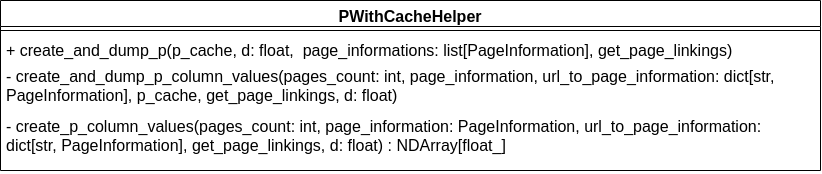
\includegraphics[keepaspectratio, width={\textwidth}]{gambar/p_with_cache_helper_class_diagram}
  \caption{\textit{Class Diagram} PWithCacheHelper}
\end{figure}

\begin{figure}[H]
  \centering
  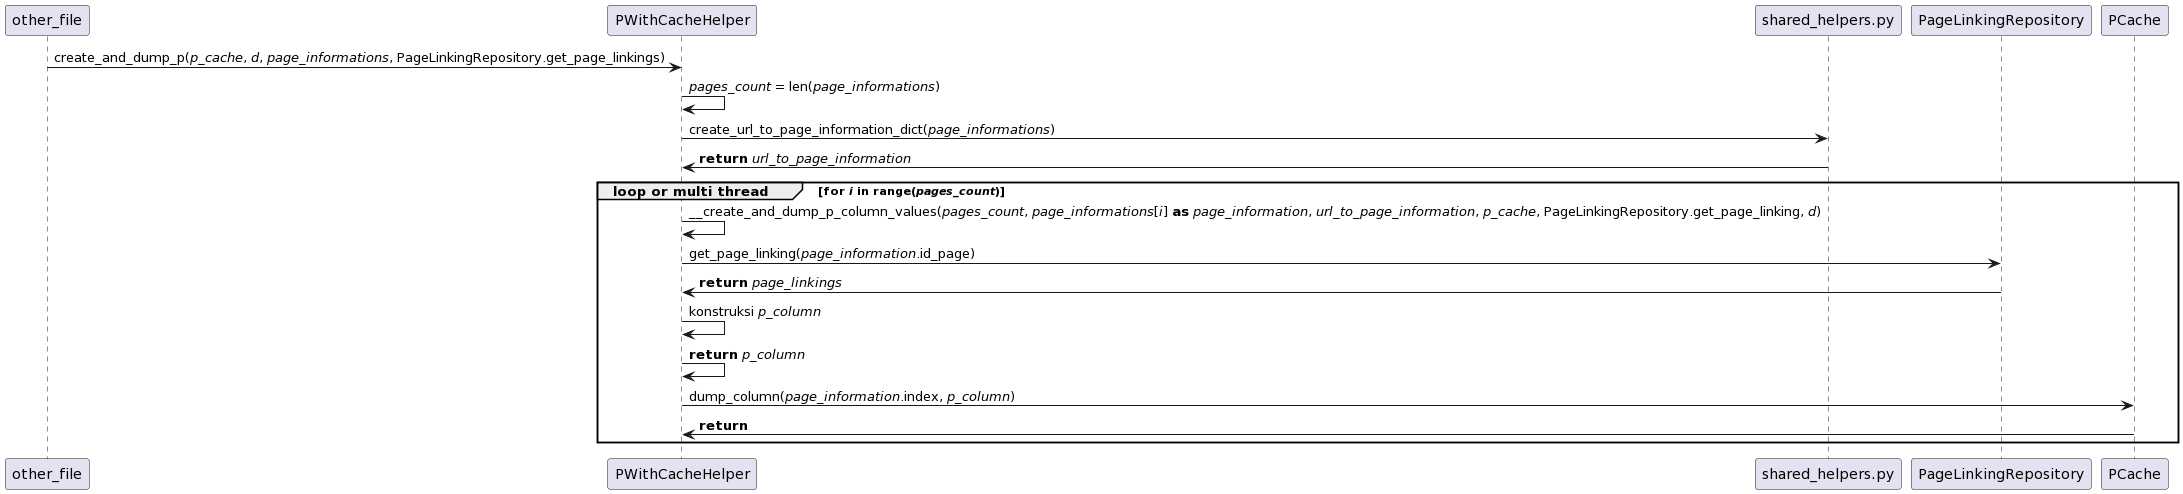
\includegraphics[width={\textwidth}, height={170px}]{gambar/p_with_cache_helper_sequence_diagram}
  \caption{Diagram alir PWithCacheHelper}
\end{figure}

Setelah matriks $P$ terbentuk menggunakan \textit{class} PWithCacheHelper, selanjutnya matriks $P$ dapat dipecah menjadi matriks $P_{ii}$ dan matriks $Q_i$. Matriks $P_{ii}$ mirip dengan matriks $Q_i$ yang merupakan matriks transisi lokal antara halaman web \textit{cluster}-$i$ terhadap \textit{cluster}-$i$, tetapi yang membedakan adalah nilai kolom dari matriks $Q_i$ sudah dinormalisasi. \textit{Class} PartitionedPHelper melalui \textit{method} \textit{dump\_partitioned\_p} memuat kolom-kolom pada matriks $P$ di PCache dipecah menjadi matriks-matriks $P_{ii}$ dimasukkan ke PiiListCache, lalu tiap kolom $P_{ii}$ dinormalisasi menjadi matriks $Q_i$ dan dimasukkan ke dalam QListCache. PiastHelper dan PastiHelper memiliki cara kerja mirip dengan PartitionedPHelper, memuat matriks $P$ dari PCache untuk dibentuk matriks $P_{i*}$ dan matriks $P_{*i}$. 

\begin{figure}[H]
  \centering
  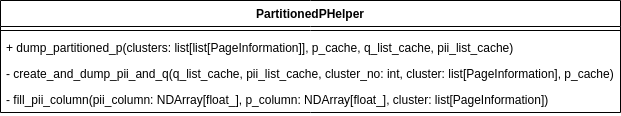
\includegraphics[keepaspectratio, width={\textwidth}]{gambar/partitioned_p_helper_class_diagram}
  \caption{\textit{Class Diagram} PartitionedPHelper}
	\label{gambar:partitioned_p_helper_class_diagram}
\end{figure}

\begin{figure}[H]
  \centering
  
\includegraphics[keepaspectratio, width={\textwidth}]{gambar/pasti_helper_class_diagram}
  \caption{\textit{Class Diagram} PastiHelper}
	\label{gambar:pasti_helper_class_diagram}
\end{figure}

\begin{figure}[H]
  \centering
  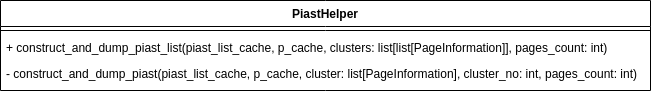
\includegraphics[keepaspectratio, width={\textwidth}]{gambar/piast_helper_class_diagram}
  \caption{\textit{Class Diagram} PiastHelper}
	\label{gambar:piast_helper_class_diagram}
\end{figure}

RPHelper bertugas menangani perkalian matriks $R$ dan matriks $P$ pada langkah \ref{alg:3.step:2:1} algoritma DPC. Alasan kenapa dibutuhkan \textit{Helper Class} untuk perkalian kedua matriks tersebut, alih-alih menggunakan operator perkalian matriks biasa, karena matriks $P$ memiliki dimensi yang besar dan harus dipecah ke dalam bentuk yang kecil, dalam penelitian ini, matriks $P$ dipecah berdasarkan kolom. Akibatnya, dalam sudut pandang program, perkalian matriks $R$ dan $P$ membutuhkan langkah-langkah kecil. Agar kode lebih rapih langkah-langkah kecil tersebut dimasukkan ke dalam \textit{class} tersendiri. Pada \textit{method} \textit{dump\_and\_mult\_rp} dilakukan \textit{looping} terhadap kolom matriks $RP$ yang nilainya masih kosong, tiap elemen dari kolom $R$ didapatkan dari perkalian antara baris matriks $R$ dan kolom matriks $P$. Hasil perkalian yaitu matriks $RP$ disimpan ke dalam \textit{class} RPCache.

\begin{figure}[H]
	\centering
	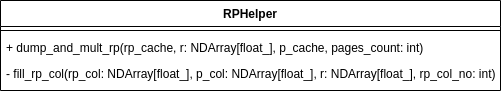
\includegraphics[keepaspectratio, width={\textwidth}]{gambar/rp_helper_class_diagram}
	\caption{\textit{Class Diagram} RPHelper}
	\label{gambar:rp_helper_class_diagram}
\end{figure}	

DPCExecutor merupakan kelas utama yang mengorkestrasi \textit{class} dan fungsi pendukung dalam mengeksekusi program DPC. Terdapat tiga \textit{public method} yang dimiliki DPCExecutor. \textit{insert\_caches} menerima \textit{class} Cache yang sudah diinstansiasi untuk disimpan ke dalam properti DPCExecutor. Selanjutnya, \textit{insert\_helpers} menerima \textit{helper class} yang sudah diinstansiasi untuk disimpan ke dalam properti DPCExecutor. Yang terakhir ada \textit{method execute} yang mengeksekusi program DPC dibantu dengan \textit{cache class} dan \textit{helper class} yang sudah dimasukkan terlebih dahulu.

Sama seperti program Pagerank yang sudah dibahas sebelumnya, program DPC dijalankan dimulai dari sebuah \textit{file} Python, \textit{run\_dpc.py}. Kode dari \textit{run\_dpc.py} dapat dilihat pada kode \ref{listing:run_dpc.py}. Langkah-langkah dari program DPC di \textit{run\_dpc.py} dapat dilihat di gambar \ref{gambar:run_dpc_sequence_diagram}. Langkah pertama dilakukan instansiasi PageInformationRepository untuk mengambil semua data PageInformation di langkah dua. PageInformation yang diambil dari PageInformationRepository, dilakukan klasterisasi pada langkah empat, hasil dari klasterisasi tersebut adalah sebuah klaster dalam bentuk \textit{hashmap}, \textit{key}-nya adalah domain, dan isinya adalah \textit{list} yang berisi PageInformation. Dari data klaster tersebut dapat dilakukan pengurutan \textit{list} PageInformation berdasarkan domain-nya di langkah enam. Selanjutnya pada langkah delapan dilakukan instansiasi PageLinkingRepository untuk mengambil data PageLinking untuk menghitung nilai dari sel matriks transisi $P$ yang dibuat pada langkah sembilan, lalu disimpan ke dalam PCache. Selanjutnya, akan dijalankan algoritma DPC di program melalui DPCExecutor. Setelah dilakukan instansiasi, pada langkah sebelas dan dua belas dimasukkan \textit{cache class} dan \textit{helper class} ke DPCExecutor. Algoritma DPC dijalankan pada langkah 13, yang secara detil dapat dilihat pada gambar \ref{gambar:dpc_executor_sequence_diagram}. Setelah selesai, dikembalikan nilai $\pi$ lalu disimpan ke basis data melalui PagerankRepository.

\begin{figure}[H]
	\centering
	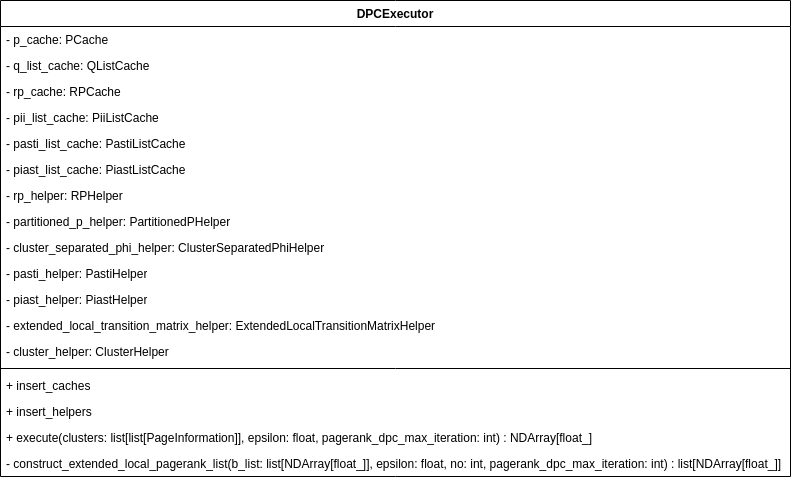
\includegraphics[keepaspectratio, width={\textwidth}]{gambar/dpc_executor_class_diagram}
	\caption{\textit{Class Diagram} DPCExecutor}
	\label{gambar:dpc_executor_class_diagram}
\end{figure}

DPCExecutor dipanggil melalui \textit{method} \textit{execute} dengan memasukan data klaster, $\epsilon$, dan max iterasi. Pertama-tama pada langkah dua sampai lima dengan data klaster dibentuk matriks $R$ dan diperoleh jumlah total halaman. Selanjutnya pada langkah enam dan tujuh, dipartisi nilai matriks $P$ yang diambil dari PCache menjadi himpunan matriks $Q$ dan $P_{ii}$. Lalu pada langkah delapan dan sembilan, dilakukan perhitungan Pagerank pada setiap halaman web yang masih terpisah pada tiap domainnya. Pada langkah sepuluh dan sebelas dilakukan perkalian matriks $R$ dan $P$. Alasan perkalian matriks $R$ dan $P$ dilakukan secara terpisah alih-alih langsung dikalikan dengan matriks $S$, karena dimensi matriks $P$ sangat besar dan nilai matriks $R$ dan $P$ tidak akan berubah, sehingga lebih baik dilakukan secara terpisah terlebih dahulu, dan disimpan ke dalam \textit{cache}. Selanjutnya pada langkah 12 sampai 15 dibentuk matriks $P_{*i}$ dan $P_{i*}$, dengan alasan yang sama dengan matriks $R$ dan $P$ yang nilainya tidak akan berubah. Setelah itu, pada langkah 16 nilai vektor $\pi$ yang masih terpisah pada tiap domainnya, disatukan tanpa ada perubahan nilai. Memasuki \textit{loop} dibentuk matriks $S$ berdasarkan nilai vektor $\pi$ yang masih terpisah terhadap domainnya. Setelah itu, dilakukan perkalian matriks $RP$ dengan matriks $S$ untuk menghasilkan matriks $A$. Matriks $A$ dapat disebut sebagai matriks transisi antara domain/klaster. Pada langkah 25, diperoleh nilai vektor $z$ dengan melakukan perhitungan Pagerank dengan masukan matriks $A$. Vektor $Z$ dapat disebut sebagai \textit{ranking} pada tiap domain. Pada langkah 26 sampai 28 dilakukan \textit{smoothing} dengan membentuk matriks \textit{extended local transition matrix} $B$, dan vektor \textit{extended local pagerank} pada setiap domain-nya. Selanjutnya pada langkah 29 nilai vektor $\pi$ diperbaharui seperti pada langkah \ref{alg:3.step:3:3} algoritma DPC. Setelah itu, nilai $\pi$ dinormalisasi pada langkah 33 dan dihitung nilai delta antara $\pi$ saat ini, dengan $\pi$ iterasi sebelumnya. Jika nilai deltanya kurang dari $\epsilon$, maka perhitungan selesai dan dikembalikan nilai $\pi$ sebagai nilai akhir. Jika tidak, kembali pada langkah awal ketika memasuki \textit{loop}, diawali dengan menambahkan variabel $iteration\_count$ dengan satu untuk menghitung jumlah iterasi yang sudah dilalui. Jumlah iterasi maksimal dapat ditentukan, apabila iterasi tidak kunjung konvergen. Jadi selain nilai delta, jumlah iterasi dapat ditentukan batasnya untuk keluar dari \textit{loop}.

\begin{figure}[H]
\centering
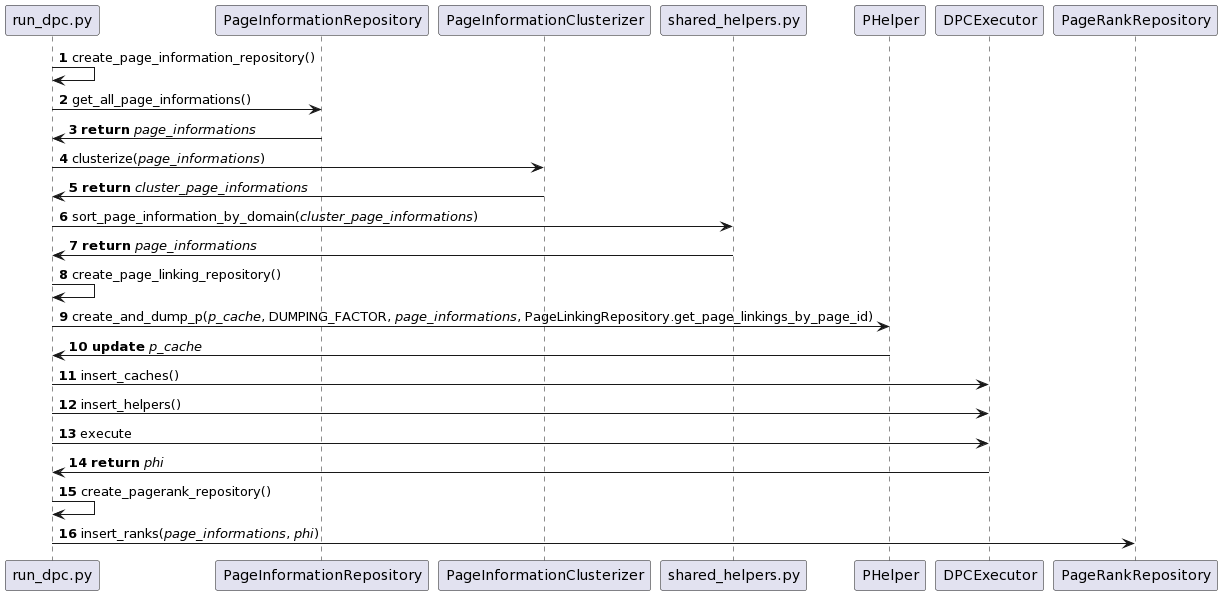
\includegraphics[width={\textheight}, height={\textwidth}, angle=270]{gambar/run_dpc_sequence_diagram}
\caption{Diagram alir \textit{run\_dpc.py}}
\label{gambar:run_dpc_sequence_diagram}
\end{figure}

\begin{figure}[H]
\centering
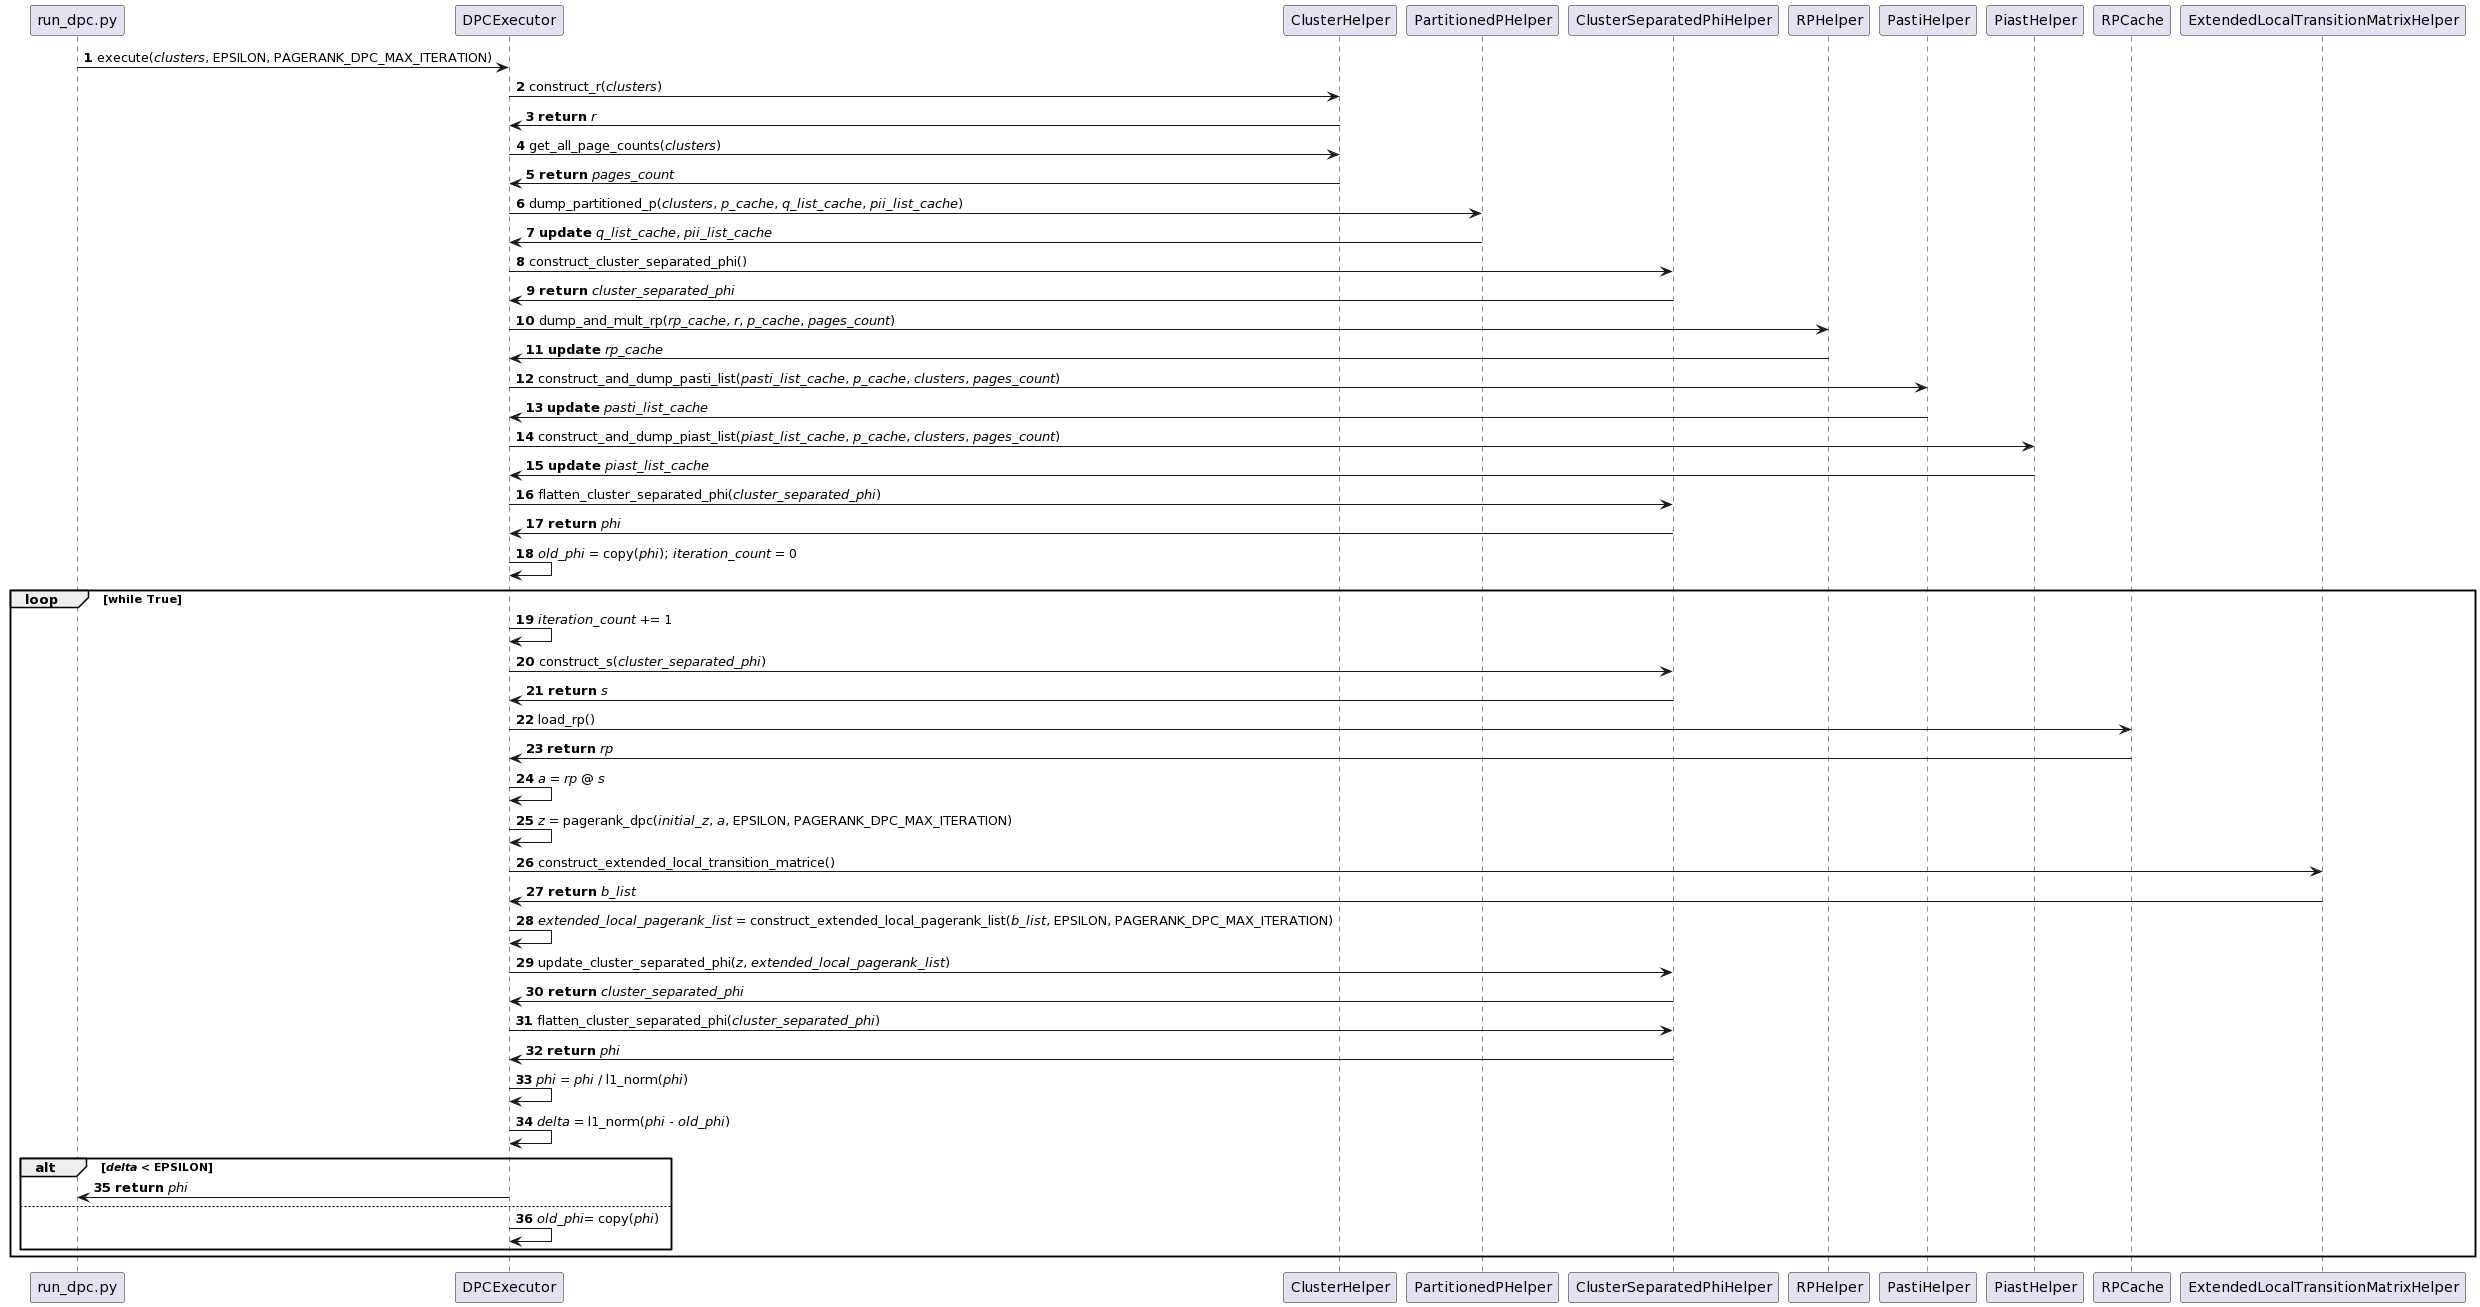
\includegraphics[width={\textheight}, height={\textwidth}, angle=270]{gambar/dpc_executor_sequence_diagram}
\caption{Diagram alir DPCExecutor}
\label{gambar:dpc_executor_sequence_diagram}
\end{figure}

\subsection{Program MDPC}

MDPC merupakan versi lebih sederhana dari algoritma DPC, sehingga kode yang dibuat sangat lebih sedikit dibanding program DPC. Selain itu juga, ada beberapa \textit{class} yang ada pada DPC juga dipakai pada program MDPC. Namun, karena matriks transisi antar \textit{cluster} $A_{mdpc}$ tidak ada pada DPC, maka dibuat \textit{class} AHelper untuk melakukan perhitungan dan membentuk matriks tersebut. Kode program dari \textit{class} AHelper dapat dilihat pada kode \ref{listing:ahelper_class}. Secara garis besar, proses pembentukan matriks $A_{mdpc}$ di \textit{class} ini dimulai dari \textit{public method} \textit{construct\_a}, dilakukan perhitungan nilai pada tiap sel matriks, lalu dilakukan normalisasi pada setiap kolom-nya. Adapun untuk dasar perhitungannya sesuai dengan persamaan \ref{eq:a_mdpc} dan dilakukan pada \textit{method \_\_sum\_sub\_transition\_matrix}.

\begin{figure}[H]
	\centering
	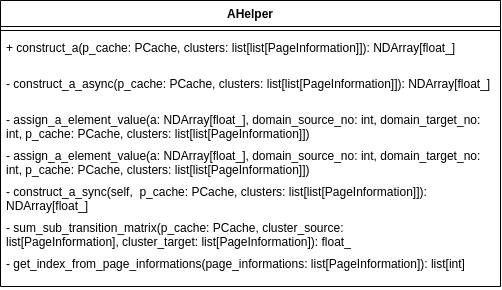
\includegraphics[keepaspectratio, width={\textwidth}]{gambar/a_helper_class_diagram}
	\caption{\textit{Class Diagram} AHelper}
\end{figure}

Selain AHelper, program MDPC juga memiliki \textit{class} ModifiedDPCV2Executor yang berperan sebagai eksekutor dari program MDPC. Secara struktur ModifiedDPCV2Executor mirip dengan \textit{class} DPCExecutor, terdapat \textit{public method insert\_caches, insert\_helpers} dan masing-masing dimulai dari \textit{public method execute}. 

\begin{figure}[H]
	\centering
	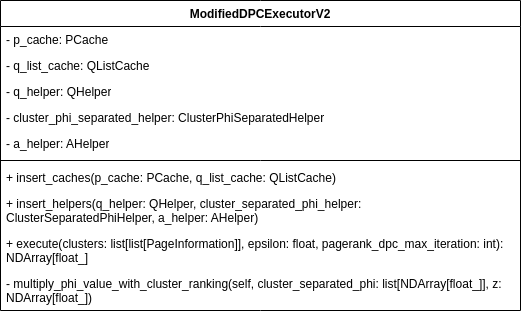
\includegraphics[keepaspectratio, width={\textwidth}]{gambar/modified_dpc_executor_v2_class_diagram}
	\caption{\textit{Class Diagram} ModifiedDPCExecutorV2}
\end{figure}

Ketika \textit{method execute} pada \textit{class} ModifiedDPCV2Executor dipanggil, hal pertama yang dilakukan adalah mengkonstruksi matriks $Q$ dan disimpan ke dalam \textit{cache}. Selanjutnya dilakukan perhitungan \textit{ranking} halaman web atau Pagerank yang masih terisolasi pada setiap domain-nya, di dalam program disimpan ke dalam variabel \textit{cluster\_separated\_phi}, sesuai dengan langkah \ref{alg:mdpc.step.1} algoritma MDPC. Setelah itu dibuat matriks transisi antar \textit{cluster} $A_{mdpc}$ menggunakan \textit{class} AHelper. Selanjutnya dilakukan perhitungan \textit{ranking} tiap \textit{cluster} dengan menggunakan $A_{mdpc}$ sebagai matriks transisi. Setelah diperoleh \textit{cluster ranking}, dilakukan perkalian \textit{ranking} halaman web yang masih terisolasi terhadap \textit{cluster} dengan \textit{cluster ranking}. Nilai Pagerank pada \textit{cluster\_separated\_phi} dianggap tidak terisolasi terhadap \textit{cluster} dan dilakukan penggabungan menjadi sebuah vektor Pagerank tunggal dan dikembalikan sebagai hasil akhir.

\begin{figure}[H]
\centering
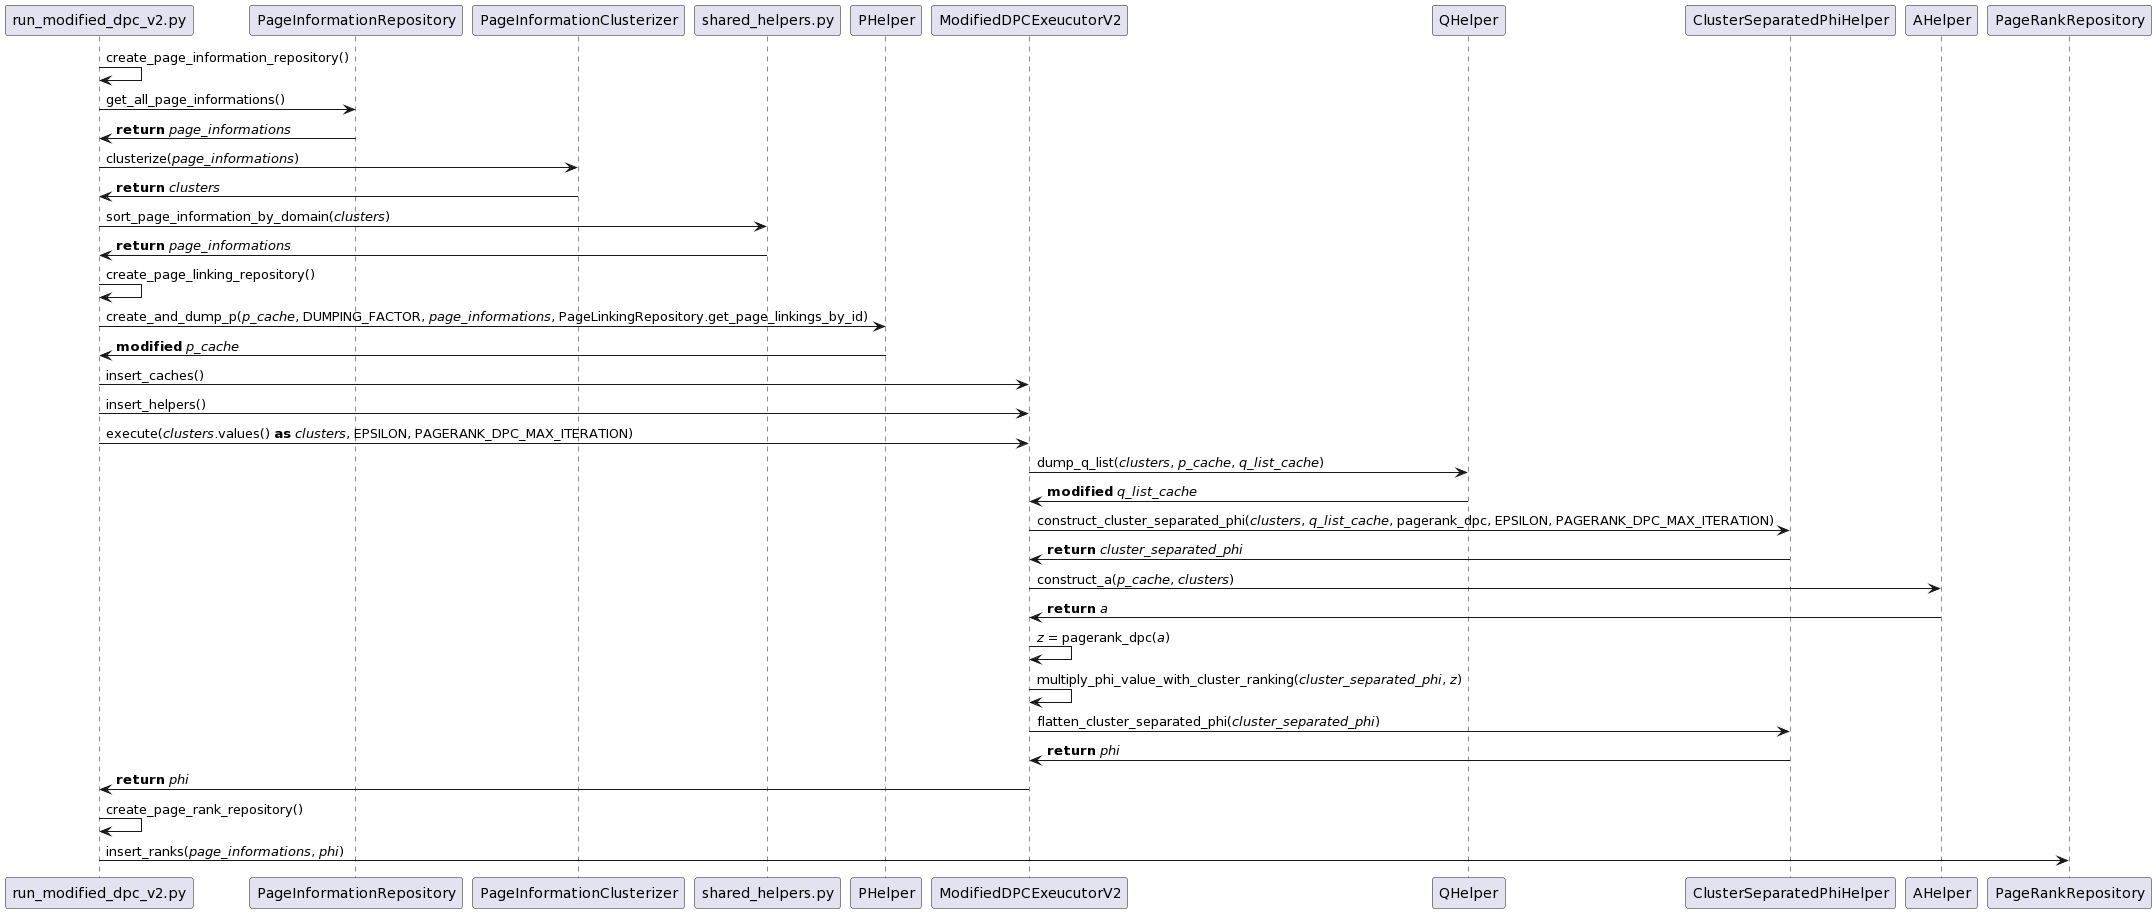
\includegraphics[width={\textheight}, height={\textwidth}, angle=270]{gambar/run_modified_dpc_v2_sequence_diagram}
\caption{Diagram alir program MDPC}
\label{gambar:run_modified_dpc_v2_sequence_diagram}
\end{figure}

Serupa dengan program DPC, program MDPC dimulai dari sebuah \textit{Python file run\_modified\_dpc\_v2.py}. Alur dari program MDPC secara keseluruhan dapat dilihat pada diagram alir gambar \ref{gambar:run_modified_dpc_v2_sequence_diagram}. Sama dengan program-program sebelumnya, langkah awal yaitu instansiasi repositori dan diambil semua data informasi halaman web PageInformation, diklasterisasi, diurutkan, dan lalu dapat dibentuk matriks $P$ yang disimpan ke dalam PCache. Selanjutnya dilakukan instansiasi \textit{cache class} dan \textit{helper class} lain lalu dimasukkan ke dalam ekskutor ModifiedDPCExecutorV2. Selanjutnya dipanggil \textit{public method execute}. Setelah diperoleh nilai $\pi$, lalu disimpan ke basis data melalui PagerankRepository.

\subsection{Program Random Walker}

\begin{figure}[H]
	\centering
	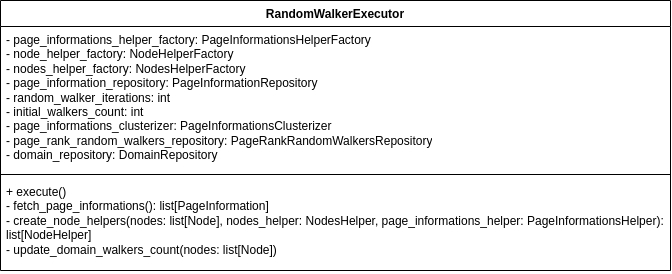
\includegraphics[keepaspectratio, width={\textwidth}]{gambar/random_walker_executor_class_diagram}
	\caption{\textit{Class Diagram} RandomWalkerExecutor}
\end{figure}

Program Random Walker merupakan sebuah simulasi dari Pagerank. Secara program, Random Walker memiliki sebuah \textit{executor class} dan beberapa \textit{factory helper} dan \textit{helper class}. Program dimulai dengan menjalankan berkas Python \textit{run\_random\_walker.py}. Berkas Python tersebut memanggil \textit{method} \textit{execute} pada \textit{class} RandomWalkerExecutor. Pertama, diambil data semua PageInformation di basis data melalui PageInformationRepository. Selanjutnya, tiap PageInformation disimpan ke dalam \textit{class} Node. Node memiliki properti \textit{page\_information}, \textit{walkers\_count} untuk menampung jumlah \textit{walker} yang berada di Node saat ini, dan \textit{next\_walkers\_count} untuk menampung jumlah \textit{walker} yang berada di Node pada iterasi selanjutnya.

\begin{figure}[H]
	\centering
	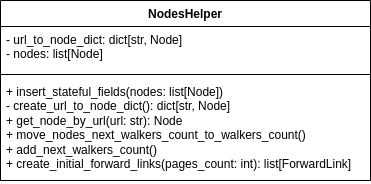
\includegraphics[keepaspectratio, width={0.55\textwidth}]{gambar/nodes_helper_class_diagram}
	\caption{\textit{Class Diagram} NodesHelper}
\end{figure}

\begin{figure}[H]
	\centering
	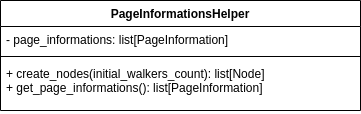
\includegraphics[keepaspectratio, width={0.55\textwidth}]{gambar/page_informations_helper_class_diagram}
	\caption{\textit{Class Diagram} PageInformationsHelper}
\end{figure}

Sebelum memasuki langkah iterasi, akan dilakukan iterasi sebanyak yang ditentukan, pada penelitian ini jumlah iterasinya adalah 20 iterasi. Memasuki iterasi, untuk setiap Node, diambil Node tujuan, dan probabilitas setiap Node tujuan. Melalui fungsi \textit{random.choices} dimasukkan jumlah \textit{walker}, \textit{list} Node tujuan, dan \textit{list} probabilitas Node tujuan. Keluaran dari fungsi \textit{random.choices} adalah \textit{list} Node dari Node tujuan sebanyak jumlah \textit{walker}, yang dianggap sebagai Node tujuan terpilih pada setiap \textit{walker}. Pada setiap Node terpilih dilakukan penambahan nilai \textit{next\_walker\_count} sebanyak satu. Setelah satu iterasi selesai, nilai \textit{walkers\_count} di-perbaharui dengan memindahkan nilai \textit{next\_walkers\_count} ke \textit{walkers\_count}. Langkah pada iterasi diulangi, sampai iterasi selesai. Penjelasan program dapat dilihat dalam bentuk diagram alir pada gambar \ref{gambar:random_walker_sequence_diagram}.

\begin{figure}[H]
	\centering
	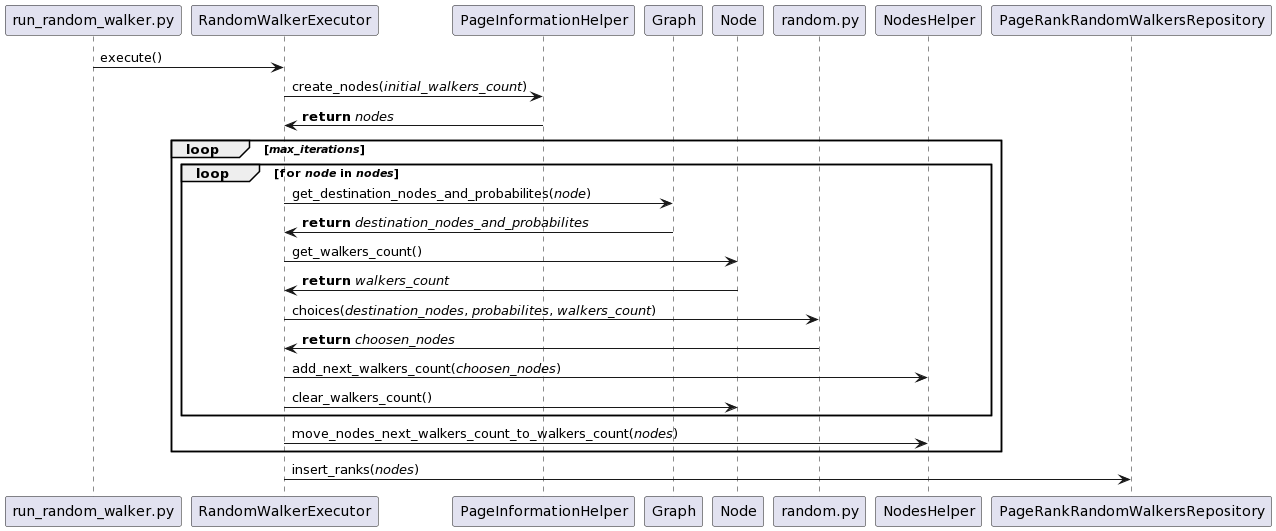
\includegraphics[width={\textheight}, height={\textwidth}, angle=270]{gambar/run_random_walker_sequence_diagram}
	\caption{Diagram alir program Random Walker}
	\label{gambar:random_walker_sequence_diagram}
\end{figure}

\section{Hasil}

Setelah program dijalankan terhadap semua \textit{dataset}, maka diperoleh hasil berikut. Pada Dataset 2 puncak penggunaan memori pada ketiga algoritma relatif sama, hal ini dikarenakan data yang cukup kecil dibandingkan \textit{overhead} memory pada program. Selanjutnya pada Dataset 1 puncak penggunaan memori terbesar ada pada algoritma pagerank asli yaitu sebesar 3,4 GB dimulai saat matriks $20.493\times 20.493$ $P$ dibentuk. Dengan perhitungan setiap sel matriks merupakan angka desimal \textit{floating point} 64bit maka besarnya matriks $P$ pada memori adalah $\pm$3,4 GB. 

Selanjutnya, pada algoritma DPC penggunaan memori terbesar adalah 842 MB yang terjadi pada pembentukan dan penyimpanan matriks $P_{*i}$ ke \textit{cache}. Mengingat domain terbesar di Dataset 1 yaitu "detik.com" dengan jumlah 2.215 halaman, maka dimensi matriks $P_{*i}$ terbesar adalah $20.493 \times 2.215$ yang akan memakan memori sebesar $\pm363$ MB, dan ketika akan disimpan ke dalam \textit{cache} menggunakan \textit{pickle library} akan dilakukan penyalinan objek sebelum ditulis ke dalam \textit{cache}, sehingga penggunaan memori $2 \times \pm363 MB = \pm726 MB$. 

Pada algoritma MDPC puncak memori sebesar $\pm86$ MB, penggunaan memori puncak terjadi pada langkah pembentukan dan penyimpanan matriks $Q$ ke \textit{cache}. Karena matriks $Q$ adalah matriks transisi lokal suatu domain, maka matriks $Q$ terbesar adalah matriks $Q$ domain "detik.com" dengan 2.215 halaman. Ukuran matriks $Q$ yang terbentuk adalah $2.215 \times 2.215$ yang secara ukuran di memori adalah $\pm39$ MB, dan di tengah proses penyimpanan ke dalam \textit{cache} dilakukan penyalinan objek sementara, sehingga ukuran memorinya menjadi dua kali lipat yaitu $\pm86$ MB. Perbandingan puncak memori dan lamanya waktu eksekusi algoritma Pagerank Original, algoritma Distributed Pagerank Computation (DPC), dan algoritma Modified DPC (MDPC), dapat dilihat pada tabel \ref{table:algorithm_performance}.

\begin{longtable}{|c|c|c|}
	\caption{Puncak penggunaan memori dan waktu eksekusi}
	\label{table:algorithm_performance} \\
	\hline
	\textbf{Algoritma} & \textbf{Puncak Penggunaan Memori(\textit{Mega Byte})} & \textbf{Waktu(Detik)} \\
	\hline
	\multicolumn{3}{|c|}{Dataset 1 (20.493 halaman)} \\
	\hline
	Pagerank & 3.417,63239 & 328,803 \\
	DPC & 842,48153 & 1.151,628 \\
	MDPC & 86,58194 & 816,375 \\
	\hline
	\multicolumn{3}{|c|}{Dataset 2 (100 halaman)} \\
	\hline
	Pagerank & 2,04511 & 0,568 \\
	DPC & 2,0563 & 19,372 \\
	MDPC & 2,05595 & 0,652 \\
	\hline
\end{longtable}

Selanjutnya akan dihitung nilai kemiripan antara nilai Pagerank yang dihasilkan program Pagerank asli, DPC, MDPC, dan Random Walker. Nilai Pagerank berbentuk vektor dan diurutkan berdasarkan \textit{id} halaman. Pada Dataset 1, nilai $KDist$ tiap vektor \textit{ranking} halaman web yang dihasilkan oleh algoritma Pagerank, DPC, MDPC, dan Random Walker dapat dilihat pada tabel \ref{table:kendall_distance_score_dataset_1}. 

\begin{longtable}{|c|c|c|c|c|}
	\caption{Nilai jarak Kendall vektor Pagerank pada dataset 1 (20.493 halaman)}
	\label{table:kendall_distance_score_dataset_1} \\
	\hline
	& \textbf{Pagerank} & \textbf{DPC} & \textbf{MDPC} & \textbf{Random Walker} \\
	\hline
	\textbf{Pagerank} & 0,0 & 0,24956 & 0,25985 & 0,02716 \\
	\hline
	\textbf{DPC} & 0,24956 & 0,0 & 0,27681 & 0,25208 \\
	\hline
	\textbf{MDPC} & 0,25985 & 0,27681 & 0,0 & 0,26387 \\
	\hline
	\textbf{Random Walker} & 0,02716 & 0,25208 & 0,26387 & 0,0 \\
	\hline
\end{longtable}

Vektor yang paling mirip atau memiliki nilai $KDist$ terkecil adalah vektor Pagerank dan Random Walker yaitu sebesar $0,02716$ atau $2,7$ persen perbedaan urutan. Sedangkan $KDist$ untuk DPC terhadap Pagerank dan Random Walker secara berurutan adalah $0,24956$ dan $0,25208$ atau $25$ persen dan $25,2$ persen perbedaan urutan. Selanjutnya untuk $KDist$ MDPC terhadap DPC, Pagerank, dan Random Walker secara berurutan adalah $0,27681$, $0,25985$, dan $0,26387$ atau $27,7$ persen, $26$ persen, dan $26,4$ persen perbedaan urutan.

Pada Dataset 2, nilai $KDist$ tiap vektor \textit{ranking} halaman web yang dihasilkan oleh algoritma Pagerank, DPC, MDPC, dan Random Walker dapat dilihat pada tabel \ref{table:kendall_distance_score_dataset_2}. Vektor yang paling mirip atau memiliki nilai $KDist$ terkecil adalah vektor Pagerank dan Random Walker yaitu sebesar $0,03293$ atau $3,3$ persen perbedaan urutan. Sedangkan $KDist$ untuk DPC terhadap Pagerank dan Random Walker secara berurutan adalah $0,17131$ dan $0,19131$ atau $17,1$ persen dan $19,1$ persen perbedaan urutan. Selanjutnya untuk $KDist$ MDPC terhadap DPC, Pagerank, dan Random Walker secara berurutan adalah $0,11091$, $0,12586$, dan $0,14949$ atau $11,1$ persen, $12,6$ persen, dan $14,9$ persen perbedaan urutan.

\begin{longtable}{|c|c|c|c|c|}
	\caption{Nilai jarak Kendall vektor Pagerank pada dataset 2 (100 halaman)}
	\label{table:kendall_distance_score_dataset_2} \\
	\hline
	& \textbf{Pagerank} & \textbf{DPC} & \textbf{MDPC} & \textbf{Random Walker} \\
	\hline
	\textbf{Pagerank} & 0,0 & 0,17131 & 0,12586 & 0,03293 \\
	\hline
	\textbf{DPC} & 0,17131 & 0,0 & 0,11091 & 0,19131 \\
	\hline
	\textbf{MDPC} & 0,12586 & 0,11091 & 0,0 & 0,14949 \\
	\hline
	\textbf{Random Walker} & 0,03293 & 0,19131 & 0,14949 & 0,0 \\
	\hline
\end{longtable}

Secara lebih detil, perbedaan peringkat halaman satu per satu berdasarkan tiap algoritmanya dapat dilihat pada tabel \ref{table:rank_comparisson_dataset_1} untuk Dataset 1, dan tabel \ref{table:rank_comparisson_dataset_2} untuk Dataset 2. Kolom \textit{Rank} menunjukan urutan peringkat halaman web, nilai pada kolom \textit{value} merupakan nilai dari peringkat halaman web yang merupakan nilai peluang ($0 \leq \text{\textit{value}} \leq 1$), dan pada nilai pada kolom \textit{page\_id} merupakan nomor pembeda atau \textit{Primary Key} yang disematkan pada basis data relasional.

\begin{longtable}{|c|c|c|c|c|}
	\caption{Perbandingan peringkat halaman web Dataset 1 (20.493 halaman) bag. 1}
	\label{table:rank_comparisson_dataset_1} \\
	\hline
	\multicolumn{5}{|c|}{Dataset 1 (20.493 halaman)} \\
	\hline
	& \multicolumn{2}{c|}{Pagerank} & \multicolumn{2}{c|}{DPC} \\
	\hline
	\textbf{Rank} & \textbf{\textit{page\_id}} & \textbf{\textit{value}} & \textbf{\textit{page\_id}} & \textbf{\textit{value}} \\
	\hline
	1 & 13.343 & 0,00975 & 9.262 & 0,00489 \\
	2 & 2.858 & 0,0093 & 9.276 & 0,00489 \\
	3 & 11.365 & 0,00635 & 9.285 & 0,00489 \\
	4 & 18.179 & 0,0048 & 16.214 & 0,00489 \\
	5 & 7 & 0,00465 & 16.217 & 0,00489 \\
	$\vdots$ & $\vdots$ & $\vdots$ & $\vdots$ & $\vdots$ \\
	20.489 & 13.012 & 0,00001 & 1.654 & 0,0 \\
	20.490 & 13.015 & 0,00001 & 1.656 & 0,0 \\
	20.491 & 13.004 & 0,00001 & 1.655 & 0,0 \\
	20.492 & 13.005 & 0,00001 & 1.653 & 0,0 \\
	20.493 & 10.723 & 0,00001 & 1.658 & 0,0 \\
	\hline
\end{longtable}

\begin{longtable}{|c|c|c|c|c|}
	\caption{Perbandingan peringkat halaman web Dataset 1 (20.493 halaman) bag. 2}
	\label{table:rank_comparisson_dataset_1} \\
	\hline
	\multicolumn{5}{|c|}{Dataset 1 (20.493 halaman)} \\
	\hline
	& \multicolumn{2}{c|}{MDPC} & \multicolumn{2}{c|}{Random Walker} \\
	\hline
	\textbf{Rank} & \textbf{\textit{page\_id}} & \textbf{\textit{value}} & \textbf{\textit{page\_id}} & \textbf{\textit{value}} \\
	\hline
	1 & 2.087 & 0,01244 & 13.343 & 0,00966 \\
	2 & 13.343 & 0,00985 & 2.858 & 0,00933 \\
	3 & 2.858 & 0,0093 & 11.365 & 0,00621 \\
	4 & 2.859 & 0,00718 & 18.179 & 0,00483 \\
	5 & 699 & 0,00654 & 7 & 0,00466 \\
	\hline
	\hline
	\multicolumn{5}{|c|}{Dataset 1 (20.493 halaman)} \\
	\hline
	& \multicolumn{2}{c|}{MDPC} & \multicolumn{2}{c|}{Random Walker} \\
	\hline
	\textbf{Rank} & \textbf{\textit{page\_id}} & \textbf{\textit{value}} & \textbf{\textit{page\_id}} & \textbf{\textit{value}} \\
	\hline
	$\vdots$ & $\vdots$ & $\vdots$ & $\vdots$ & $\vdots$ \\
	20.489 & 16.464 & 0,0 & 9.192 & 0,00001 \\
	20.490 & 16.504 & 0,0 & 9.167 & 0,00001 \\
	20.491 & 15.644 & 0,0 & 16.005 & 0,00001 \\
	20.492 & 13.898 & 0,0 & 9.179 & 0,00001 \\
	20.493 & 16.347 & 0,0 & 15.866 & 0,00001 \\
	\hline
\end{longtable}

\begin{longtable}{|c|c|c|c|c|}
	\caption{Perbandingan peringkat halaman web Dataset 2 (100 halaman) bag. 1}
	\label{table:rank_comparisson_dataset_2} \\
	\hline
	\multicolumn{5}{|c|}{Dataset 2 (100 halaman)} \\
	\hline
	& \multicolumn{2}{c|}{Pagerank} & \multicolumn{2}{c|}{DPC} \\
	\hline
	\textbf{Rank} & \textbf{\textit{page\_id}} & \textbf{\textit{value}} & \textbf{\textit{page\_id}} & \textbf{\textit{value}} \\
	1 & 72 & 0,08431 & 72 & 0,1306 \\
	2 & 62 & 0,01856 & 95 & 0,02583 \\
	3 & 54 & 0,01856 & 91 & 0,02583 \\
	4 & 55 & 0,01856 & 87 & 0,02583 \\
	5 & 59 & 0,01856 & 97 & 0,02583 \\
	$\vdots$ & $\vdots$ & $\vdots$ & $\vdots$ & $\vdots$ \\
	96 & 63 & 0,00199 & 1 & 0,00043 \\
	97 & 64 & 0,00199 & 25 & 0,00037 \\
	98 & 80 & 0,00199 & 63 & 0,00037 \\
	99 & 28 & 0,00184 & 64 & 0,00037 \\
	100 & 1 & 0,0015 & 80 & 0,00037 \\
	\hline
\end{longtable}

\begin{longtable}{|c|c|c|c|c|}
	\caption{Perbandingan peringkat halaman web Dataset 2 (100 halaman) bag. 2}
	\label{table:rank_comparisson_dataset_2} \\
	\hline
	\multicolumn{5}{|c|}{Dataset 2 (100 halaman)} \\
	\hline
	& \multicolumn{2}{c|}{MDPC} & \multicolumn{2}{c|}{Random Walker} \\
	\hline
	\textbf{Rank} & \textbf{\textit{page\_id}} & \textbf{\textit{value}} & \textbf{\textit{page\_id}} & \textbf{\textit{value}} \\
	\hline
	1 & 72 & 0,16809 & 72 & 0,08381 \\
	2 & 54 & 0,03158 & 54 & 0,01856 \\
	3 & 55 & 0,03158 & 62 & 0,01847 \\
	4 & 59 & 0,03158 & 55 & 0,01847 \\
	5 & 62 & 0,03158 & 59 & 0,01842 \\
	$\vdots$ & $\vdots$ & $\vdots$ & $\vdots$ & $\vdots$ \\
	96 & 25 & 0,00048 & 80 & 0,002 \\
	97 & 63 & 0,00048 & 63 & 0,00198 \\
	98 & 64 & 0,00048 & 64 & 0,00197 \\
	99 & 80 & 0,00048 & 28 & 0,0018 \\
	100 & 1 & 0,00022 & 1 & 0,00151 \\
	\hline
\end{longtable}

Selain perbedaan nilai peringkat, perbedaan selisih nilai atau hasil pengurangan antara pada setiap halaman web antara algoritma satu dengan yang lainnya dapat dilihat pada tabel \ref{table:rank_value_difference_dataset_1_part_1} dan tabel \ref{table:rank_value_difference_dataset_1_part_2} untuk Dataset 1, dan tabel \ref{table:rank_value_difference_dataset_2_part_1} dan tabel \ref{table:rank_value_difference_dataset_2_part_2} untuk Dataset 2. Mengetahui perbedaan selisih nilai penting untuk mengetahui seberapa jauh deviasi atau perubahan hasil nilai \textit{ranking} antara keempat algoritma (Pagerank Original, DPC, MDPC, dan Random Walker). Semakin besar nilai selisihnya, semakin besar pula perbedaannya. Hal ini juga merupakan keniscayaan karena perbedaan algoritma yang dipakai. Namun, umumnya, selisih yang dibawah $10^{-5}$ dapat ditoleransi dan dianggap sama. Oleh karena itu nilai yang ditampilkan di tabel hanya lima angka desimal, atau lima angka di belakang koma.
 
\begin{longtable}{|c|c|c|c|}
	\caption{Selisih nilai peringkat halaman web Dataset 1 (20.493 halaman) Bagian 1}
	\label{table:rank_value_difference_dataset_1_part_1} \\
	\hline
	\multicolumn{4}{|c|}{Dataset 1 (20.493 halaman)} \\
	\hline
	\textbf{\textit{page\_id}} & \textbf{Pagerank - DPC} & \textbf{Pagerank - MDPC} & \textbf{DPC - MDPC} \\
	\hline
	1 & 0,00002 & 0,00001 & 0,0  \\
	2 & 0,00245 & 0,00008 & 0,00237  \\
	3 & 0,00245 & 0,00008 & 0,00237  \\
	4 & 0,00251 & 0,00217 & 0,00034  \\
	5 & 0,00244 & 0,0019 & 0,00054  \\
	$\vdots$ & $\vdots$ & $\vdots$ & $\vdots$ \\
	20.490 & 0,00006 & 0,00001 & 0,00005  \\
	20.491 & 0,00003 & 0,00003 & 0,0  \\
	20.492 & 0,00003 & 0,00003 & 0,0  \\
	20.493 & 0,00006 & 0,00001 & 0,00005  \\
	20.494 & 0,00003 & 0,00003 & 0,0  \\
	\hline
\end{longtable}

\begin{longtable}{|c|c|c|c|}
	\caption{Selisih nilai peringkat halaman web Dataset 1 (20.493 halaman) bagian 2. Ket: Random Walker (RW)}
	\label{table:rank_value_difference_dataset_1_part_2} \\
	\hline
	\multicolumn{4}{|c|}{Dataset 1 (20.493 halaman)} \\
	\hline
	\textbf{\textit{page\_id}} & \textbf{RW - Pagerank} & \textbf{RW - DPC} & \textbf{RW - MDPC} \\
	\hline
	1 & 0,0 & 0,00002 & 0,00001  \\
	2 & 0,00001 & 0,00246 & 0,00009  \\
	3 & 0,0 & 0,00246 & 0,00008  \\
	4 & 0,00001 & 0,00252 & 0,00218  \\
	5 & 0,0 & 0,00244 & 0,0019  \\
	$\vdots$ & $\vdots$ & $\vdots$ & $\vdots$ \\
	\hline
	\hline
	\multicolumn{4}{|c|}{Dataset 1 (20.493 halaman)} \\
	\hline
	\textbf{\textit{page\_id}} & \textbf{RW - Pagerank} & \textbf{RW - DPC} & \textbf{RW - MDPC} \\
	\hline
	20.490 & 0,0 & 0,00005 & 0,0  \\
	20.491 & 0,0 & 0,00003 & 0,00003  \\
	20.492 & 0,0 & 0,00003 & 0,00003  \\
	20.493 & 0,0 & 0,00005 & 0,0  \\
	20.494 & 0,0 & 0,00003 & 0,00003  \\
	\hline
\end{longtable}

Selanjutnya akan ditampilkan perbedaan selisih keempat algoritma pada Dataset 2 yang berisi 100 halaman web. Sama dengan tabel untuk Dataset 1, angka yang ditampilkan di bawah hanya lima angka di belakang koma.

\begin{longtable}{|c|c|c|c|}
	\caption{Selisih nilai peringkat halaman web Dataset 2 (100 halaman) bagian 1}
	\label{table:rank_value_difference_dataset_2_part_1} \\
	\hline
	\multicolumn{4}{|c|}{Dataset 2 (100 halaman)} \\
	\hline
	\textbf{\textit{page\_id}} & \textbf{Pagerank - DPC} & \textbf{Pagerank - MDPC} & \textbf{DPC - MDPC} \\
	\hline
	1 & 0,00107 & 0,00128 & 0,00021  \\
	2 & 0,00088 & 0,00112 & 0,00024  \\
	3 & 0,00156 & 0,00314 & 0,0047  \\
	4 & 0,00571 & 0,00079 & 0,00492  \\
	5 & 0,00571 & 0,00079 & 0,00492  \\
	$\vdots$ & $\vdots$ & $\vdots$ & $\vdots$ \\
	96 & 0,00269 & 0,00257 & 0,00012  \\
	97 & 0,00784 & 0,00038 & 0,00746  \\
	98 & 0,00328 & 0,00482 & 0,0081  \\
	99 & 0,00328 & 0,00348 & 0,0002  \\
	100 & 0,00277 & 0,00244 & 0,00033  \\
	\hline
\end{longtable}

\begin{longtable}{|c|c|c|c|}
	\caption{Selisih nilai peringkat halaman web Dataset 2 (100 halaman) bagian 2. Ket: Random Walker (RW)}
	\label{table:rank_value_difference_dataset_2_part_2} \\
	\hline
	\multicolumn{4}{|c|}{Dataset 2 (100 halaman)} \\
	\hline
	\textbf{\textit{page\_id}} & \textbf{RW - Pagerank} & \textbf{RW - DPC} & \textbf{RW - MDPC} \\
	\hline
	1 & 0,00001 & 0,00108 & 0,00128  \\
	2 & 0,00001 & 0,00089 & 0,00113  \\
	3 & 0,00001 & 0,00157 & 0,00313  \\
	4 & 0,00004 & 0,00576 & 0,00083  \\
	5 & 0,00008 & 0,00563 & 0,00071  \\
	$\vdots$ & $\vdots$ & $\vdots$ & $\vdots$ \\
	96 & 0,00004 & 0,00266 & 0,00253  \\
	97 & 0,00004 & 0,0078 & 0,00033  \\
	98 & 0,00001 & 0,00327 & 0,00483  \\
	99 & 0,00008 & 0,00336 & 0,00356  \\
	100 & 0,0 & 0,00278 & 0,00244  \\
	\hline
\end{longtable}

Perbedaan hasil cukup signifikan antara Distributed Pagerank Computation (DPC) dan Modified DPC (MDPC) terhadap Pagerank Original dan Random Walker disebabkan karena dasar dari perhitungannya yang berbeda. DPC dan MDPC memisahkan halaman web berdasarkan domain-nya, sedangkan Pagerank dan Random Walker melakukan perhitungan secara utuh.

Dapat disimpulkan, algoritma Pagerank Original paling cepat dan paling mirip hasilnya dengan algoritma Random Walker dalam melakukan pe-\textit{ranking}-an halaman web, namun memerlukan memori utama yang lebih besar. Sedangkan algoritma DPC dan MDPC memerlukan memori utama lebih kecil, sehingga cocok untuk komputer satu mesin dengan memori utama terbatas, tetapi dengan konsekuensi perbedaan hasil yang cukup besar terhadap algoritma Pagerank Original dan algoritma Random Walker dan waktu eksekusi yang lebih lambat.